\chapter{Informative Seafloor Exploration}
\lhead{Informative Seafloor Exploration}
\label{Informative-Seafloor-Exploration}

	The Gaussian process based inference model for benthic habitat mapping devised in Chapter \ref{Benthic-Habitat-Mapping} provides a Bayesian framework for habitat inference and prediction. With such an inference model, this chapter proceeds to develop an informative path planning policy for benthic habitat mapping.
	
	The outset of this chapter begins by motivating the need for a measure of mutual information (section \ref{Informative-Seafloor-Exploration:Mutual-Information}). Such a measure would allow inference based on the \textit{essential} information contained in any given sub-region of interest. The mutual information criterion can then be employed as the acquisition function for informative path planning, in order to evaluate thus compare the desirability of visiting candidate regions and locations.
	
%	Two mutual information criterion are investigated in this thesis - Monte Carlo Joint Predictive Information Entropy (section \ref{Informative-Seafloor-Exploration:MCJPIE}) and Linearised Model Differential Entropy (section \ref{Informative-Seafloor-Exploration:LMDE}).
	
	As Gaussian process classifiers lack analytical forms for the predictive joint distribution of target labels, any mutual information measure derived from the predictive joint distribution must rely on numerical estimation techniques. As such, estimating joint prediction information entropy requires a Monte Carlo sampling based approach. Section \ref{Informative-Seafloor-Exploration:MCJPIE} describes such a mutual information criterion, hereby named Monte Carlo Joint Predictive Information Entropy (MCJPIE).
	
	However, a Monte Carlo approach suffers some several drawbacks, such as computational complexity and limited estimation accuracy. Instead, this thesis proposes a new and alternative mutual information measure, Linearised Model Differential Entropy (LMDE), that is more computationally tractable than MCJPIE. Section \ref{Informative-Seafloor-Exploration:LMDE} defines and derives LMDE, and demonstrates its ability to capture uncertainty in both variance and bias.
	
	Section \ref{Informative-Seafloor-Exploration:Receding-Horizon-Formulation} then formulates a receding horizon approach to informative path planning. This provides a simple yet effective framework for a large scale exploration task such as seafloor exploration for benthic habitat mapping. In particular, the receding horizon formulation strikes a balance between exploring in a non-myopic way and doing so with reasonable tractability constraints.
	
	Finally, section \ref{Informative-Seafloor-Exploration:Informative-Exploration-over-Scott-Reef-Seafloor} assesses the performance of various approaches to informative seafloor exploration for benthic habitat mapping. Multiple acquisition criterions are tested under both the receding horizon approach and a myopic greedy approach, which verifies the benefits of linearised model differential entropy under the receding horizon formulation. Under a mapping accuracy criterion, simulations over the Scott Reef dataset demonstrates that LMDE acquisition outperform other acquisition criterions.
	
	\section{Mutual Information}
	\label{Informative-Seafloor-Exploration:Mutual-Information}
		
		In order to devise an informative path planning policy, it is important to select an appropriate acquisition criterion which measures the desirability of traversing a particular candidate path. Section \ref{Background:Related-Work} provided an outline of related investigations on various acquisition functions for informative path planning in the benthic habitat mapping context. 
		
		Much of the intractability discussed in such literature can trace its reason down to the fact that benthic habitat mapping is a classification problem instead of a regression problem. While Gaussian process regression provide analytical forms for inference, due to a non-Gaussian likelihood response, Gaussian process classification is no longer analytically tractable. Instead, several approximations must be made, which were discussed in section \ref{Background:GaussianProcesses:Classification}.
		
		This thesis addresses the tractability status of the problem through proposing an alternative acquisition criterion that captures mutual information. In the current literature, acquisition criterion either do not directly capture mutual information, such as \eqref{Equation:AsherBenderAcquisitionCriterion}, or take too long to compute due to required estimations from sampling, such as \eqref{Equation:KrauseAcquisitionCriterion}. 
		
		Instead, linearised differential entropy (LMDE) as an acquisition function captures an appropriate form of mutual information. Specifically, it regularises between reducing mutual bias and mutual uncertainty through taking advantage of both the latent mean and covariance structure, as well as the non-Gaussian likelihood response. Tractability of the approach is further improved through a linearisation approximation on such an acquisition criterion.
		
		
%		\subsection{Motivation}
%		
%			For both modeling purposes and path planning purposes, simply knowing the entropy at each query point is not enough. 
%			
%		\subsection{Shannon Entropy}
%		
%		\subsection{Lack of a Closed Form Solution}
		
	\section{Monte Carlo Joint Predictive Information Entropy}
	\label{Informative-Seafloor-Exploration:MCJPIE}
			Provide pseudocode for limited and good way of doing it
			
		\subsection{Binary Classification}
		
		\subsection{Multiclass Classification}
		
	\section{Linearised Model Differential Entropy}
	\label{Informative-Seafloor-Exploration:LMDE}
	
		In this section we introduce the linearised differential entropy of Gaussian process classifiers. This method attempts to address the need for a measure of mutual entropy that is more computationally viable compared to Monte Carlo methods. We motivate the properties that such a measure is desired to have, and proceed to define, and derive, such a measure. Finally, we discuss its interpretation and visualise its advantage through simple tests cases in both the binary and multiclass classification setting.
		
		\subsection{Binary Classification}
	
			For binary classification, linearisation is performed on the likelihood response function.
		
			Suppose we have trained our Gaussian process classifier using Laplace approximation with respect to a training set $\mathcal{D} = \{X, \bvec{y}\} = \{[ \bvec{x}_{1}, \bvec{x}_{2}, \dots, \bvec{x}_{n}]^{T}, [y_{1}, y_{2}, \dots, y_{n}]\}$ with $n$ training points. We know that the latent function $f(\bvec{x})$ is distributed as a GP with a particular predictive mean $m(\bvec{x})$ and covariance $k(\bvec{x}, \bvec{x}')$ once conditioned on the training data \eqref{Section:LinearisedEntropy:Equation:PredictiveGP}. From here on we omit explicitly notating the training set that was conditioned upon.
			
			\begin{equation}
				f(\bvec{x}) \sim \mathcal{GP}(m(\bvec{x}), k(\bvec{x}, \bvec{x}'))
			\label{Section:LinearisedEntropy:Equation:PredictiveGP}
			\end{equation}
			
			Let $X^{\star} = [ \bvec{x}^{\star}_{1}, \bvec{x}^{\star}_{2}, \dots, \bvec{x}^{\star}_{n^{\star}}]^{T}$ denote the collection of $n^{\star}$ query points for which inference is to be performed upon. Denote $\bvec{f}^{\star}$ the vector of latent function values $f^{\star}_{i} = f(\bvec{x}^{\star}_{i})$ at each query point. We have by definition of a GP that $\bvec{f}^{\star}$ is multivariate Gaussian distributed with corresponding means $\mu^{\star}_{i} = m(\bvec{x}^{\star}_{i})$ and covariances $\Sigma^{\star}_{ij} = k(\bvec{x}^{\star}_{i}, \bvec{x}^{\star}_{j})$ \eqref{Section:LinearisedEntropy:Equation:PredictiveGaussianDistribution}.
			
			\begin{equation}
				\bvec{f}^{\star} = [f^{\star}_{1}, f^{\star}_{2}, \dots, f^{\star}_{n^{\star}}]^{T} \sim \mathcal{N}(\vec{\upmu}^{\star}, \Sigma^{\star})
			\label{Section:LinearisedEntropy:Equation:PredictiveGaussianDistribution}
			\end{equation}
				
			The binary prediction probability $\vec{\uppi^{\star}}$ at the query points is obtained through passing the queried latent function random vector $\bvec{f}^{\star}$ through a response function in a component wise fashion \eqref{Section:LinearisedEntropy:Equation:Response}.
			
			\begin{equation}
				\vec{\uppi}^{\star} = \vec{\upsigma}(\bvec{f}^{\star})\mathrm{ \quad i.e. \;\;}\pi^{\star}_{i} = \sigma(f^{\star}_{i}) \quad \forall i \in \{1, 2, \dots, n^{\star}\}
			\label{Section:LinearisedEntropy:Equation:Response}
			\end{equation}
			
			As a straightforward transformation of the latent vector, the predictive probability vector $\vec{\uppi^{\star}}$ is thus a random vector itself. The usual procedure is then to treat the expected prediction probabilities $\mathbb{E}[\vec{\uppi^{\star}}]$ as the posterior class probabilities for further inference. However, this discards any information regarding the joint behaviour of an arbitrary collection of query points. As a result, a measure of mutual information shared amongst the query points cannot be obtained.
			
			One straightforward approach to address this problem is to perform Monte Carlo estimation of the posterior joint distribution for class predictions via jointly sampling latent vectors from the GP, assigning class label 1 for positive latent values and -1 otherwise, and compute the Shannon entropy \cite{ShannonEntropy} from the estimated joint distribution. Aside from the time complexity required for sampling enough draws for accurate joint distribution estimation, Monte Carlo estimated Joint Information Entropy (MCJIE) also has the tendency to over-represent uncertainties under small samples.
					
			Instead, we propose using the joint distribution of the predictive probabilities $\vec{\uppi^{\star}}$ itself as a basis of constructing a measure of mutual information. Unlike traditional approaches where inference depends only on the expectance $\mathbb{E}[\vec{\uppi^{\star}}]$ such that structural information from the latent GP is compromised, we utilise also the covariance $\mathbb{V}[\vec{\uppi^{\star}}]$, which contains information regarding both the latent GP and the response likelihood.
		
			\begin{figure}[!htbp]
				\centering
					\includegraphics[width = 0.6\linewidth]{Figures/linearisation.eps}
				\caption{Linearisation accuracy for a probit response: Green shade represents the latent variance while blue shade represents the predictive variance. Gold lines show local linearisation about latent expectance.}
				\label{Figure:Linearisation}
			\end{figure}
				
			As the predictive probabilities are nonlinear transformations of the Gaussian distributed latent vector, they are no longer Gaussian distributed. In order to retain analytical tractability, we propose linearising the response function about the latent expectance $\bar{f}^{\star}_{i} := \mathbb{E}[f^{\star}_{i}]$. Figure \ref{Figure:Linearisation} illustrates the linearisation accuracy for a probit response. Observe that points with latent expectance far away from zero translate to near zero predictive variance even under high latent variance. Linearisation is thus very accurate for those points. For points with latent expectances near zero, we require the latent variances to be sufficiently small for linearisation to be accurate.
			
			\subsubsection{Derivation}
			
				We proceed to derive the linearisation which also serves to construct the definition of linearised differential entropy. With first order Taylor expansion, we linearise the response about the latent mean $\bar{f}^{\star}_{i} = \mathbb{E}[f^{\star}_{i}]$ \eqref{Section:LinearisedEntropy:Equation:LinearisingSigmoid}. \begin{equation}
					\sigma(f^{\star}_{i}) \approx \sigma_{L}(f^{\star}_{i}) := \sigma(\bar{f}^{\star}_{i}) + \sigma'(\bar{f}^{\star}_{i}) (f^{\star}_{i} - \bar{f}^{\star}_{i})
				\label{Section:LinearisedEntropy:Equation:LinearisingSigmoid}
				\end{equation}
				
				The prediction probabilities are now approximated as a linear transformation $\sigma_{L}(f)$ of the latent vector, so that it is also multivariate Gaussian distributed with expectance and covariance available in analytical form \eqref{Section:LinearisedEntropy:Equation:MomentsLinearisedSigmoid}. \begin{align*}
				\numberthis \label{Section:LinearisedEntropy:Equation:MomentsLinearisedSigmoid}
						\vec{\upsigma}_{L}(\bvec{f}^{\star}) & \sim \mathcal{N}(\vec{\upmu}^{\star}_{L}, \Sigma^{\star}_{L}) \\
						({\mu^{\star}_{L}})_{i} & = \mathbb{E}[\sigma_{L}(f^{\star}_{i})] = \sigma(\bar{f}^{\star}_{i}) \\
						({\Sigma^{\star}_{L}})_{ij} & = \mathbb{C}\mathrm{ov}[\sigma_{L}(f^{\star}_{i}), \sigma_{L}(f^{\star}_{j})] = \sigma'(\bar{f}^{\star}_{i}) \sigma'(\bar{f}^{\star}_{j}) \mathbb{C}\mathrm{ov}[f^{\star}_{i}, f^{\star}_{j}]
				\end{align*}
				
				We then define the linearised differential entropy $H^{\star}_{L}$ at the query points $X^{\star}$ to be the differential entropy for which the random vector $\vec{\upsigma}_{L}(\bvec{f}^{\star})$ holds. Since $\vec{\upsigma}_{L}(\bvec{f}^{\star})$ is multivariate Gaussian distributed, $H_{L}$ exhibits a closed form \eqref{Section:LinearisedEntropy:Equation:BinaryLinearisedEntropy}. \begin{equation}
					H^{\star}_{L} := \frac{1}{2} \log\Big((2 \pi e)^{n^{\star}} \det(\Sigma^{\star}_{L})\Big)
				\label{Section:LinearisedEntropy:Equation:BinaryLinearisedEntropy}
				\end{equation}			
						
		\subsection{Multiclass Classification}
				
			For multiclass classification, linearisation is performed on the softmax function $\sigma^{m}$ which returns the corresponding predictive class probability $\vec{\uppi}^{m}$ for class $m \in \{1, 2, \dots, c\}$ \eqref{Section:LinearisedEntropy:Equation:Softmax} \cite{GaussianProcessForMachineLearning}. For notational clarity we move the query star ($^\star$) to the left and use the superscript $m$ to index the classes. The latent vector $\bvec{f}_{i} := \{f^{m}_{i}\}_{m \in \{1, 2, \dots, c\}}$ represents the collection of $c$ latent values across classes at the query point $i$, and is distinct from $\bvec{f}^{m} := \{f^{m}_{i}\}_{i \in \{1, 2, \dots, n^{\star}\}}$ which represents the collection of $n^{\star}$ latent values across query points for class $m$. \begin{equation}
				^{\star}\pi^{m}_{i} = \sigma^{m}(^{\star}\bvec{f}_{i}) := \frac{\exp(^{\star}f^{m}_{i})}{\sum_{l = 1}^{c} \exp(^{\star}f^{l}_{i})} \qquad m \in \{1, 2, \dots, c\}
			\label{Section:LinearisedEntropy:Equation:Softmax}
			\end{equation}
			
			In this derivation, we focus on the case of OVA, or one versus all, multiclass classification, where each class is trained against all other classes independently with a binary classifier. For $c$ classes, $c$ binary classifiers are trained independently and also performs inference independently. The normalisation is then inherently captured in the softmax \eqref{Section:LinearisedEntropy:Equation:Softmax}. This approach avoids the Monte Carlo sampling step in the inference stage of a typical GP multiclass classifier under Laplace Approximation \cite{GaussianProcessForMachineLearning}, and is thus faster in computational time. Furthermore, because each classifier is trained independently, both the learning stage and the inference stage can be performed in parallel, further speeding up the process in a way that was not available under the original scheme. This is important later in under a receding horizon formulation, where the inference stage is included in the objective function of an optimiser such that repeated evaluations would benefit dramatically from shorter inference time.
			
			\subsubsection{Derivation}
			
				Similar to the binary case, to linearise we first find the gradient of each of the $c$ softmax functions \eqref{Section:LinearisedEntropy:Equation:SoftmaxGradient}. For notational simplicity, the query stars ($^{\star}$) are omitted in this derivation except for $n^{\star}$.
				
				\begin{equation}
					\frac{\partial \sigma^{m}}{\partial f^{k}_{i}}(\bvec{f}_{i}) =
					\begin{cases} 
						- \frac{\exp(f^{m}_{i}) \exp(f^{k}_{i})}{\sum_{l = 1}^{c} \exp(f^{l}_{i})} & \text{for } k \neq m  \\
						- \frac{\exp(f^{m}_{i})^{2}}{\big(\sum_{l = 1}^{c} \exp(f^{l}_{i})\big)^{2}} + \frac{\exp(f^{m}_{i})}{\sum_{l = 1}^{c} \exp(f^{l}_{i})}& \text{for } k = m
					\end{cases}
				\label{Section:LinearisedEntropy:Equation:SoftmaxGradient}
				\end{equation}			
			
				The numerators are explicitly left in the form of products of exponentiation instead of exponentiation of sums to reflect ways to cache quantities during computation. 
				
				Hence, for each class $m$ at query point $i$ we compute a softmax gradient vector \eqref{Section:LinearisedEntropy:Equation:SoftmaxGradientVector}.
				
				\begin{equation}
					\frac{\partial \sigma^{m}}{\partial \bvec{f}_{i}}(\bvec{f}_{i}) := \begin{bmatrix} \frac{\partial \sigma^{m}}{\partial f^{1}_{i}}(\bvec{f}_{i}) & \frac{\partial \sigma^{m}}{\partial f^{2}_{i}}(\bvec{f}_{i}) & \dots & \frac{\partial \sigma^{m}}{\partial f^{c}_{i}}(\bvec{f}_{i}) \end{bmatrix}^{T}
				\label{Section:LinearisedEntropy:Equation:SoftmaxGradientVector}
				\end{equation}
				
				The linearisation is again performed on the mean latent predictions $\bar{\bvec{f}}_{i} = \mathbb{E}[\bvec{f}_{i}]$ so that the we can approximate the softmax $\sigma^{m}(\bvec{f}_{i})$ with the linearised softmax $\sigma^{m}_{L}(\bvec{f}_{i})$ \eqref{Section:LinearisedEntropy:Equation:LinearisedSoftmax} in an analogous form as \eqref{Section:LinearisedEntropy:Equation:LinearisingSigmoid}.
				
				\begin{equation}
					\begin{aligned}
						\sigma^{m}(\bvec{f}_{i}) \approx \sigma^{m}_{L}(\bvec{f}_{i}) & := \sigma^{m}(\bar{\bvec{f}}_{i}) + \left. \frac{\partial \sigma^{m}}{\partial \bvec{f}_{i}} \right|^{T}_{\bvec{f}_{i} = \bar{\bvec{f}}_{i}} (\bvec{f}_{i} - \bar{\bvec{f}}_{i}) \\
						& = \bvec{c}^{m}_{i} + (\bvec{g}^{m}_{i})^{T} (\bvec{f}_{i} - \bar{\bvec{f}}_{i})
					\end{aligned}
				\label{Section:LinearisedEntropy:Equation:LinearisedSoftmax}
				\end{equation}
				
				where we have notated the constants $\bvec{c}^{m}_{i} := \sigma^{m}(\bar{\bvec{f}}_{i})$ and $\bvec{g}^{m}_{i} := \frac{\partial \sigma^{m}}{\partial \bvec{f}_{i}}(\bar{\bvec{f}}_{i})$.
				
				To determine the distribution of the vector of softmax values across query points, we first define the following \eqref{Section:LinearisedEntropy:Equation:Definitions}.
				
				\begin{equation}
					\begin{aligned}
						F &:= \{f^{m}_{i}\}_{m \in \{1, 2, \dots, c\}, i \in \{1, 2, \dots, n^{\star}\}} \in \mathbb{R}^{c \times n^{\star}} \\
						\vec{\upsigma}^{m}_{L}(F) &:= \begin{bmatrix} \sigma^{m}_{L}(\bvec{f}_{1}) & \sigma^{m}_{L}(\bvec{f}_{2}) & \dots & \sigma^{m}_{L}(\bvec{f}_{n}) \end{bmatrix}^{T}
					\end{aligned}
				\label{Section:LinearisedEntropy:Equation:Definitions}
				\end{equation}
							
				We can now compute the covariance of the linearised sigmoid of a particular class $m$ between two query points $i$ and $j$, as well as the expectance at a particular query point $i$ \eqref{Section:LinearisedEntropy:Equation:MomentsLinearisedSoftmax}.
				
				\begin{align*}
				\numberthis \label{Section:LinearisedEntropy:Equation:MomentsLinearisedSoftmax}
						\vec{\upsigma}^{m}_{L}(F) & \sim \mathcal{N}(\vec{\upmu}^{m}_{L}, \Sigma^{m}_{L}) \\
						(\mu^{m}_{L})_{i} & = \mathbb{E}[\sigma^{m}_{L}(\bvec{f}_{i})] =  \sigma^{m}(\bar{\bvec{f}}_{i}) \\
						(\Sigma^{m}_{L})_{ij} & = \mathbb{C}\mathrm{ov}[\sigma^{m}_{L}(\bvec{f}_{i}), \sigma^{m}_{L}(\bvec{f}_{i})] \\
						& = \mathbb{C}\mathrm{ov}[(\bvec{g}^{m}_{i})^{T} \bvec{f}_{i}, (\bvec{g}^{m}_{j})^{T} \bvec{f}_{j}] \\
						& = \sum_{k = 1}^{c} (g^{m}_{i})^{k} (g^{m}_{j})^{k} \mathbb{C}\mathrm{ov}[f^{k}_{i}, f^{k}_{j}]
				\end{align*}
							
				where $(g^{m}_{i})^{k}$ denotes the $k^{\text{th}}$ element of $\bvec{g}^{m}_{i}$. The last equality arises as a result of employing OVA multiclass classification, where latent values of classes $k$ and $l$, $k \neq l$, are conditionally independent given training observations.
				
				Finally, we define the linearised entropy of the OVA multiclass Gaussian process classifier as follows \eqref{Section:LinearisedEntropy:Equation:MulticlassLinearisedEntropy}.
				
				\begin{equation}
					H_{L} := \frac{1}{2} \log\Bigg((2 \pi e)^{n^{\star}} \det\bigg(\sum_{m = 1}^{c} \Sigma^{m}_{L}\bigg)\Bigg)
				\label{Section:LinearisedEntropy:Equation:MulticlassLinearisedEntropy}
				\end{equation}			
		
		\subsection{Interpretation of Model Differential Entropy}
		
			It is worthwhile to remember that linearised differential entropy is not an approximation to the usual prediction information entropy - the former is a differential entropy on a multivariate Gaussian distribution and the latter is an information entropy on the distribution of discrete class predictions combinations, which is a multivariate multinomial distribution. They have different interpretations and both can have advantageous properties under different scenarios. We propose using linearised differential entropy as an alternative acquisition function for informative path planning which can be more beneficial under specific exploration purposes.
			
			Specifically, while the prediction information entropy (PIE) represents the confidence in the model, the linearised differential entropy (LDE) represents the the separability of classes in the feature space. In fact, LDE quantifies the ambiguity of the predictive probabilities. In particular, it is possible for GP multiclass classifiers to conclude low predictive variance even under uncertain predictive probabilities. In this case, the LDE would be high while the PIE would be low at such locations, indicating that the model is confident about its inability to separate classes \cite{AsherBender}. Similar to the bias-variance trade-off, such a situation indicate high bias, and is distinct from a model that is unconfident about its ability to separate classes, which would correspond to high variance. This demonstrates that PIE and LDE are two complementary measures of entropy that can assist each other in identifying both places of high bias and high variance.
			
			In the case of informative path planning, a measure of mutual information is required. While the formulation of LDE readily incorporates joint distributions \eqref{Section:LinearisedEntropy:Equation:MulticlassLinearisedEntropy}, to obtain the joint PIE one would need to perform estimations from techniques such as Monte Carlo sampling. We refer to the latter as Monte Carlo estimated Joint Information Entropy (MCJIE).
			
			Here we compare linearised differential entropy and the usual prediction information entropy of a Gaussian process classifier. For visualisation purposes, only the marginalised entropies across the feature space are shown. We show examples where abundant information is available, so that the difference in the properties in the two measures can be emphasized. 
			
			Figure \ref{Figure:Results:BinaryLinearisedEntropy} shows a simple binary classification problem with abundant data on features $x_{1}$ and $x_{2}$, allowing a misclassification rate of 2.155\%. The classifier is trained with an axis aligned Gaussian kernel with a probit response under Laplace approximation. 
	
			\begin{figure}[t]
			\centering
				\includegraphics[width = \linewidth]{Figures/binary.eps}
			\caption{GP binary classifier: prediction information entropy and linearised differential entropy under abundant data}
			\label{Figure:Results:BinaryLinearisedEntropy}
			\end{figure}
			
			In this example, there are no training points around the edges shown. As a result, the GP classifier learns a slightly lower signal to noise ratio in the latent function, and bounces back to its latent GP prior for which it remains uncertain regarding class label assignments. The prediction information entropy reflects this change more rapidly, so that it is high both at the decision boundaries and wherever observations are lacking. If the acquisition function for informative exploration is a function of the prediction information entropy, the vehicle would be suggested to explore both places with lacking observations and the decision boundaries. 
			
			On the other hand, linearised differential entropy focuses on the decision boundary as it is constructed to be only high when the latent function is near zero (figure \ref{Figure:Linearisation}). We can see in Figure \ref{Figure:Results:BinaryLinearisedEntropy} that the linearised differential entropy emphasizes on where the latent expectance is close to zero, and filters out the rest. If the linearised differential entropy is used as the acquisition function, the vehicle would focus on the decision boundaries within the feature space. Notice that regions far away from observations in the feature space are also assigned with high linearised differential entropy, as the latent function bounces back to its prior, so that the vehicle would explore those parts of the feature space if necessary.
			
	%		Intuitively, under abundant data, we would like the classifier to only indicate high entropies at decision boundaries. In Figure \ref{Figure:Results:BinaryLinearisedEntropy}, we see that the prediction information entropy is indeed near its maximum at the predict decision boundaries. As an artefact of the Laplace approximation, however, it is also quite high around the edges where the classifier has learned a slightly lower signal to noise ratio. As there are no data points around the edges, the GP classifier learns a latent function that bounces back to its latent GP prior for which it remains uncertain regarding the class labels. 
			
	%		This suggests that if the prediction information entropy is used as the acquisition function for path planning, the vehicle would be suggested to spent some time travelling around the region of interest, collecting data it is already expecting. The prediction entropy is high at both predicted decision boundaries and also places with lower relative data density compared. 
	%		
	%		This leads to the classic exploration-exploitation dilemma most machine learning algorithms face. It is possible that there exists decision boundaries yet to be detected at regions of lower relative data density. Is it worth it for the vehicle to explore and discover such regions, or exploit the currently known boundaries and map it better? In most exploration applications, the priority is to map the region of interest as accurately and fast as possible in order to reduce time and cost. While it is possible that there exists undiscovered decision boundaries at regions of lower relative data density, it is undesirable under cost constraints that this possibility is weighed heavily by the vehicle even under abundant data.
			
			This demonstrates the advantage of linearised differential entropy. We can see in Figure \ref{Figure:Results:BinaryLinearisedEntropy} that the linearised differential entropy is only high at the predicted decision boundaries. Note that the colour scale has been centred around zero differential entropy. Under such an acquisition function, the vehicle would focus strictly on the mapping the predicted decision boundaries better.
			
			Figure \ref{Figure:Results:MulticlassLinearisedEntropy} shows a similar scenario with a multi-class scenario with 4 labels. The same behaviour as the binary case is observed, where the linearised differential entropy approach pushes down the entropy level of all regions except the predicted decision boundaries.
		
			\begin{figure}[t]
			\centering
				\includegraphics[width = \linewidth]{Figures/multiclass.eps}
			\caption{GP multiclass classifier: prediction information entropy and linearised differential entropy under abundant data}
			\label{Figure:Results:MulticlassLinearisedEntropy}
			\end{figure}
				
	%		In the case of a feature space that does not contain the spatial coordinates for which path planning in based on, the MCJIE method may spent a lot of time in a single region where it is locally rich in span of a subspace of the feature space. However, this is suboptimal as this means it is giving up on trying to go for other regions that may have an even richer span of the feature space. The linearised differential entropy method focuses its efforts (prioritises) the decision boundaries in the feature space at the expense of overlooking regions with less observations. This leads to smoother paths as it will look at all elements of the feature space. As long as one of the features is spatially correlated (depth in our case), this will lead to smoother paths.
		
	\section{The Receding Horizon Formulation}
	\label{Informative-Seafloor-Exploration:Receding-Horizon-Formulation}
	
		In this section we present a receding horizon approach to the informative path-planning problem. Specifically, we use the linearised differential entropy derived earlier as the acquisition function. We motivate the use of the approach and discuss its structure.
		
		The receding horizon approach is inspired by the philosophy of model predictive control (MPC) in control theory, for which a continuous problem is discretised such that an optimal control problem is transcribed into a static optimisation problem at each time step. Similar to MPC, while receding horizon methods are almost always suboptimal, it provides a computationally tractable approach that is rather stable in performance. Furthermore, a receding horizon approach avoids a myopic and greedy approach to informative path planning. Myopic approaches often result in the vehicle fixating on a region with local maximum entropy due to its inability to sacrifice immediate rewards for future rewards in a faraway region. Lastly, a receding horizon approach is simple to implement and sufficient for most missions for which strict optimality is not necessary.
		
	%		Informative path planning is a highly dynamical process in which the observations the vehicle decides to take can significantly impact the belief space of the vehicle and hence alter its action. As a result, Gaussian processes are often used for modeling the environment for which path planning is to be performed. The tractability of Gaussian processes regression allows sophisticated methods for informative path planning, such as  performing sequential Bayesian optimisation to achieve informative path planning over continuous domains \cite{Roman:SequentialBayesianOptimisation}. One desired property we would like to achieve with an informative path-planning problem is that the search is non-myopic. When the objective is to collect data on a particular spatial phenomenon, Gaussian process regression can be used as the model under which strong theoretical performance guarantees can be made \cite{Meliou:2007:NIP:1619645.1619742}. However, in the case where the objective is to collect data in the form of discrete labels, a Gaussian process classifier is used instead for modeling the phenomenon. As discussed earlier, the joint entropy from a Gaussian process classifier is not available in closed form. Instead, another measure of joint entropy was developed in the previous section which demonstrated desired properties for informative exploration. To take advantage of the tractability of linearised differential entropy over finite collections of query points, we discretise the spatial domain and select paths composed of finitely many query points. The acquisition criterion is then set to be the linearised differential entropy of the query points that compose the path.
	

		
		\subsection{Formulation and Structure}
	
			The receding horizon approach requires the selection of a horizon length and the number of control points (query points) for which the path is to be defined upon. The horizon length plays a significant role in the performance of the method. A short horizon length tends to produce paths that are similar to a myopic approach. A horizon length that is too long, however, can be both inefficient and destabilising. For an informative path-planning scenario, looking ahead too far can have diminishing returns in its informativeness, as the vehicle's belief space would be significantly altered by the time it was supposed to follow the original proposed path.
	
	%		\begin{figure}[!htbp]
	%		\centering
	%			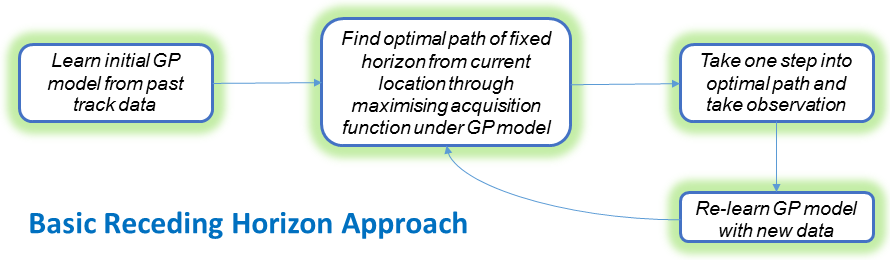
\includegraphics[width = \linewidth]{Figures/receding_horizon_informative_path_planning.png}
	%		\caption{Basic Receding Horizon Structure}
	%		\label{Figure:Results:RecedingHorizonMethodOutline}
	%		\end{figure}
		
			\begin{figure}[!htbp]
				\begin{center}
				\smartdiagramset{planet font = \small, satellite font = \scriptsize, planet color = orange!60, planet size = 2cm, satellite size = 2 cm, distance planet-satellite = 3.5cm}
				\smartdiagram[connected constellation diagram]
				{Receding Horizon Path Planning, Learn GP model from collected data, Compute finite optimal path, Move to first control point, Record observation}
				\end{center}
%				\begin{center}
%					\smartdiagramset{text width = 3cm}
%					% \smartdiagramset{set color list = {orange!50, green!80, blue!50}}
%					\smartdiagram[circular diagram:clockwise]{Learn GP model from collected data, Compute finite optimal path, Move to first control point \& record observation}
%				\end{center}
			\caption{Basic Receding Horizon Structure}
			\label{Figure:Results:RecedingHorizonMethodOutline}
			\end{figure}
					
			Figure \ref{Figure:Results:RecedingHorizonMethodOutline} describes the basic flow of the receding horizon approach approach, which resembles the technique of model predictive control (MPC) in control theory. That is, it computes an optimal policy of finite horizon in each time step, and only executes the first action from the policy. The acquisition function to be maximised in each step is flexible, and we compare LDE acquisition \eqref{Section:LinearisedEntropy:Equation:MulticlassLinearisedEntropy} against MCJIE acquisition and other acquisition functions under the receding horizon structure in the next section. In each time step, a new path of a certain horizon length is proposed, which is discretised into a finite set of control points. The vehicle only executes the policy towards the first control point while recording observations. It then relearns the GP classifier model with new observations, and repeats the process. 
	
%			Provide a flow diagram?
	
%			Horizon Length
%			
			Step Spacing
				
		\subsection{Implementation}

			Path Generation \& Natural Coordinates
			
			Turn Angle Limits for Smooth Paths
			
			Feature Space Transformations
			
		\subsection{Computational Aspects: Optimisation Process and Bottlenecks}
		
		Feasibility and Practicality of LMDE emphasized here
		
		\subsection{Computational Aspects: Model Update}
	
%	\section{Results with Abundant Uniform Test Data Set}
%	
%	\section{Results with Scarce Uniform Test Data Set}
%	
%	\section{Results with Simulated Track Data}
	
	\section{Informative Exploration over Scott Reef Seafloor}
	\label{Informative-Seafloor-Exploration:Informative-Exploration-over-Scott-Reef-Seafloor}
	
		\subsection{Ground Truth Generation}
		
		\subsection{Practical Considerations}
		
		\subsection{Entropy and Prediction Maps}
		
		\subsection{Performance Assessment}
	
	
	